%----------------------------------------------------------------------------------------
%	PACKAGES AND OTHER DOCUMENT CONFIGURATIONS
%----------------------------------------------------------------------------------------

\documentclass[paper=a4, fontsize=11pt]{scrartcl} % A4 paper and 11pt font size
\usepackage[a4paper, left=2.5cm, right=2cm, top=2cm, bottom=2cm]{geometry}
\linespread{1.2}

\usepackage[utf8]{inputenc}
\addtokomafont{disposition}{\rmfamily}
\usepackage{polski} % Język polski/hyphenation
\usepackage{amsmath,amsfonts,amsthm} % Math packages
\usepackage{indentfirst}
\usepackage{graphicx}
\usepackage{caption}
\usepackage{flafter}


\def \thesis {Aplikacja uczenia maszynowego metodą SVM}
\def \author {Pavlo Boidachenko}
\def \department {Wydział Fizyki, Astronomii i Informatyki Stosowanej}

\usepackage{sectsty} % Allows customizing section commands
%\allsections{\mdseries\itshape} % Make all sections centered, the default font and small caps

\usepackage{fancyhdr} % Custom headers and footers
\pagestyle{fancy} % Makes all pages in the document conform to the custom headers and footers
\fancyhead[L]{\textbf{Praca licencjacka:} \thesis} % No page header - if you want one, create it in the same way as the footers below
\fancyhead[C]{}
\fancyhead[R]{}
\fancyfoot[L]{\author} % left footer
\fancyfoot[C]{\thepage} % center footer
\fancyfoot[R]{} % right footer
\renewcommand{\headrulewidth}{0.3pt} % Remove header underlines
\renewcommand{\footrulewidth}{0.3pt} % Remove footer underlines
\setlength{\headheight}{14.06pt} % Customize the height of the header

\usepackage[style=alphabetic,sorting=nyt,sortcites=true,autopunct=true,babel=hyphen,hyperref=true,abbreviate=false,backref=true,backend=biber]{biblatex}
\addbibresource{ref.bib}

\numberwithin{equation}{section} % Number equations within sections (i.e. 1.1, 1.2, 2.1, 2.2 instead of 1, 2, 3, 4)
\numberwithin{figure}{section} % Number figures within sections (i.e. 1.1, 1.2, 2.1, 2.2 instead of 1, 2, 3, 4)
\renewcommand{\thetable}{\Roman{table}}

\setlength\parindent{10pt} % Removes all indentation from paragraphs - comment this line for an assignment with lots of text

\newcommand{\horrule}[1]{\rule{\linewidth}{#1}} % Create horizontal rule command with 1 argument of height
\newcommand*{\captionsource}[2]{%
  \caption[{#1}]{%
    #1%
    \\\hspace{\linewidth}%
    Źródło: #2%
  }%
}

%Other packages
\usepackage{multirow}
\usepackage{url}
\usepackage{bm}
\usepackage{xcolor}
\definecolor{Black}{RGB}{0,0,0}
\definecolor{Red}{RGB}{255,0,0}
\definecolor{Blue}{RGB}{0,0,255}
\definecolor{Green}{RGB}{0,255,0}
\definecolor{Gray}{RGB}{45,45,45}
\definecolor{linkcol}{RGB}{57,0,155}
\usepackage[unicode, pdftex, colorlinks=true, urlcolor=Gray, linkcolor=Gray, citecolor=Gray]{hyperref}

\usepackage{tocloft}
\renewcommand{\cftsecleader}{\cftdotfill{\cftdotsep}}

\begin{document}

\thispagestyle{empty}
\begin{titlepage}
    \begin{center}
        \Large \textbf{Uniwersytet Jagielloński w Krakowie}\vspace{0.2cm}\\ \department\\
        \vspace*{1cm} 
        \vspace{3cm}
        \Large
        \textbf{\author}\\\vspace{0.5cm}
        \normalsize Nr albumu: 1124969\\
        \vspace{2cm}
        \Huge
        \textbf{\thesis}

        \vspace{1.5cm}
        \normalsize
        Praca licencjacka\\
        na kierunku informatyki\\ \vspace{0.15cm}
        \vfill
        \vspace{2cm}
        \begin{minipage}{1\textwidth}
            \begin{flushright}
                Praca wykonana pod kierunkiem\\
                dr Grzegorz Surówka\\
                Department of Information Technologies
            \end{flushright}
        \end{minipage}
        \vspace{2cm}
        \begin{center}
            Kraków 2019
        \end{center}
    \end{center}

\end{titlepage}

\newpage 
 \thispagestyle{empty}
\vspace{2.5cm}
\begin{flushleft}
\large \textbf{Oświadczenie autora pracy}\vspace{0.6cm}\\
\end{flushleft}

\noindent Świadom odpowiedzialności prawnej oświadczam, że niniejsza praca dyplomowa została napisana przeze mnie samodzielnie i nie zawiera treści uzyskanych w sposób niezgodny z obowiązującymi przepisami.\\

\noindent Oświadczam również, że przedstawiona praca nie była wcześniej przedmiotem procedur związanych z uzyskaniem tytułu zawodowego w wyższej uczelni.
\vspace{2cm}
\begin{center}
    \begin{tabular}{lr}
        ................................~~~~~~~~~~~~~~~~~~~~~~~~~~~~~~~~~~~~~~&
        .......................................... \\
        {~~~~Kraków, dnia} & {Podpis autora pracy~~~~}
    \end{tabular}
\end{center}
\vspace{5cm}
\begin{flushleft}
    \large \textbf{Oświadczenie kierującego pracą}
\end{flushleft}

\noindent Potwierdzam, że niniejsza praca została przygotowana pod moim kierunkiem i~kwalifikuje się do przedstawienia jej w postępowaniu o nadanie tytułu zawodowego.
\vspace{2cm}
\begin{center}
    \begin{tabular}{lr}
        ................................~~~~~~~~~~~~~~~~~~~~~~~~~~~~~~~~~~~~~~&
        ............................................ \\
        {~~~~Kraków, dnia} & {Podpis kierującego pracą~~}
    \end{tabular}
\end{center}
\vfill
\newpage
\tableofcontents
\newpage

\section{Wstęp} % SECTION
\subsection{Motywacja}
    \par W aktualne czasy temat Uczenia Maszynowego jest popularny\ref{fig:google-trends-ml} jak nigdy do tego. 
    Projekty z użyciem Uczenia Maszynowego pozwalają na tworzenie aplikacji które
    jeszcze 10 lat temu trudno było wyobrazić.
\begin{figure}[h]
    \begin{center}
        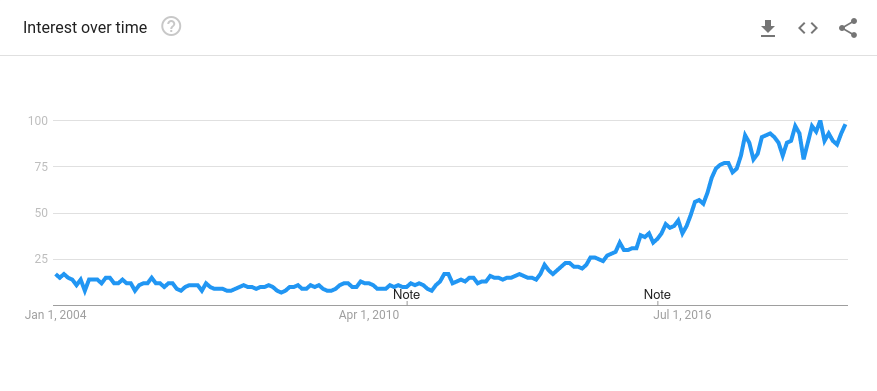
\includegraphics[scale=0.5]{./img/google-trends-ml.png}
        \captionsource{Machine Learning trends}{Google Trends}
        \label{fig:google-trends-ml}
    \end{center}
\end{figure}
    \par Rozpowszechnienie Uczenia Maszynowego również spowodowało i moje zainteresowanie tematem.
    Z tego powodu dla swojej pracy licencjackiej wybrałem temat: Aplikacja uczenia maszynowego 
    metodą SVM.  Po zakończeniu pracy spodziewam się podwyższyć swoją kompetencje w dziale 
    Uczenia Maszynowego.
\subsection{Cel}
    \par Celem mojej pracy licencjackiej jest stworzenie oprogramowania pozwalającego na generowanie
    modeli używając Maszyny wektorów nośnych\textit{(ang. Support Vector Machine, SVM)} z graficznym 
    interfejsem użytkownika.  Program będą mogli użyć osoby potrzebujące szybko przetrenować kilka 
    modeli, przetestować ich dla różnych parametrów, zwizualizować dane. Program ma na celu ułatwienie
    pracę z Maszyną wektorów nośnych poprzez graficzny interfejs użytkownika
    oparty na bibliotekę QT. Część funkcjonalna programu jest oparta o bibliotekę LIBSVM\cite{CC01a}.
\subsection{Zakres}
    Program powinien móc ustawiać parametry dla wybranej metody oraz jądra\textit(ang. kernel), 
    generować wykresy podawanych zbiorów danych, interpretować różne formaty zbiorów danych, 
    wykonywać Sprawdzian krzyżowy (ang. Cross validation, CV), mieć metodę do optymalizacji 
    parametrów, pokazywać wyniki trenowania oraz testowania modeli.
    \newpage
\section{Metoda klasyfikacji SVM} % SECTION
\subsection{Opis}
    \par Swój program napisałem w oparciu o bibliotekę LIBSVM\cite{CC01a}. Maszyna Wektorów
    Nośnych(ang. Support Vector Machine. SVM) - klasyfikator, nauka którego ma na celu 
    wyznaczenie hiperpłaszczyzny rozdzielającej dwie klasy z maksymalnym marginesem. 
    LIBSVM implementuje pięć typów Maszyny Wektorów Nośnych: C-SVC, $\mu$-SVC, One class SVM,
    $\epsilon$-SVR, $\mu$-SVR.
\subsection{C-SVC}
    \par C-Support Vector Classification
\subsection{$\mu$-SVM}
\subsection{Kernel}
\newpage
\section{Projekt aplikacji} % SECTION
\subsection{Opis}
\subsection{Technologie}
\newpage
\section{Podsumowanie} % SECTION
\subsection{Odniesienie do celu pracy}
\subsection{Co można dodać}

\newpage
\nocite{*}
\printbibliography

\end{document}
